%%%%%%%%%%%%%%%%%%%%%%%%%%%%%%%%%%%%%%%%%%%%%%%%%%%%%%%%%%%%%%%%%%%%%%%%%%%%%%%%%%%%%%%%%%%%%%%%%%%%%%%%%%%%%%%%%%%%%%%%%%%%%%%%%%%%%%%%%%%%%%%%%%%%%%%%%%%%%%%%%%%%%%%%%%%%%%%%%%%%%%%%%%%%%%%%%%%%%%%%%%%%%%%%%%%%%%%%%%%%%%%%%%%
%%%%%%%%%%%%%%%%%%%%%%%%%%%%%%%%%%%%%%%%%%%%%%%%%%%%%%%%%%%%%%%%%%%%%%%%%%%%%%%%%%%%%%%%%%%%%%%%%%%%%%%%%%%%%%%%%%%%%%%%%%%%%%%%%%%%%%%%%%%%%%%%%%%%%%%%%%%%%%%%%%%%%%%%%%%%%%%%%%%%%%%%%%%%%%%%%%%%%%%%%%%%%%%%%%%%%%%%%%%%%%%%%%%
%%%%%%%%%%%%%%%%%%%%%%%%%%%%%%%%%%%%%%%%%%%%%%%%%%%%%%%%%%%%%%%%%%%%%%%%%%%%%%%%%%%%%%%%%%%%%%%%%%%%%%%%%%%%%%%%%%%%%%%%%%%%%%%%%%%%%%%%%%%%%%%%%%%%%%%%%%%%%%%%%%%%%%%%%%%%%%%%%%%%%%%%%%%%%%%%%%%%%%%%%%%%%%%%%%%%%%%%%%%%%%%%%%%
\chapter{The Large Hadron Collider}

The Large Hadron Collider (LHC)~\cite{bib:LHC_machine_2008,bib:LHC_2004} is a particle accelerator installed in the former LEP~\cite{bib:LEP_design_1984} tunnel at CERN~\cite{bib:CERN:web}.
It is 26.7\km in circumference and consists of two separate rings, which are, in periods of operation, inhabited by two counter-circulating beams.
At the interaction points of the two beams, either proton-proton collisions or heavy ion collisions take place.
In this thesis, only $pp$-collision data from the year 2012 is analysed.
Thus, all machine values cited in the following chapters and paragraphs refer to the setup for $pp$-collisions in 2012 if not stated otherwise.

The beams are separated into bunches which rotate with a bunch spacing of 50\ns corresponding to a collision frequency of 20\mhz.
Before the bunches are actually filled into the LHC ring they are pre-accelerated in other accelerators, which are in the order they are actually passed by the protons: Linac2, Proton  Synchrotron Booster (PSB), Proton Synchrotron (PS), Super Proton Synchrotron (SPS).
The injector chain and the LHC ring with its experiments is visualised in Fig~\ref{fig:LHC}.
\begin{figure}[!b]
  \centering
      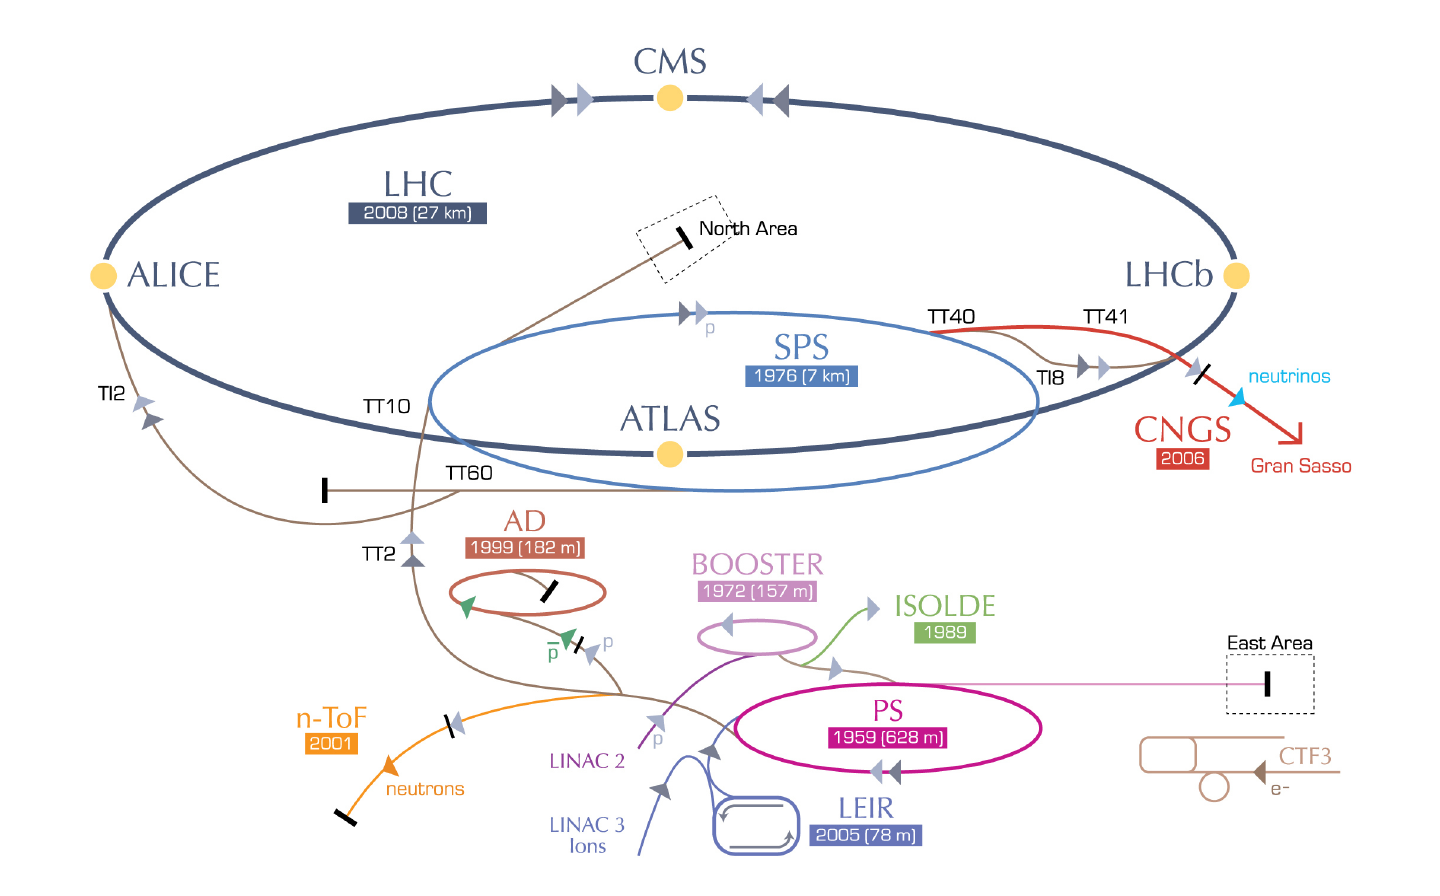
\includegraphics[width=0.90\textwidth]{figures/experiment/LHC/LHC_small.png}
  \caption{Visualisation of the LHC with its experiments and the injector chain. Taken from~\cite{bib:CERNBrochure}.}  
  \label{fig:LHC}
\end{figure}

In the LHC, the beams are kept on their circular path with the help of a magnetic field of 4.76\tesla.
Further quadrupole and sextupole magnets squeeze and focus the bunches resulting in a bunch spread of roughly 8\cm length and a Gaussian shape radius of 20\mum RMS at the interaction point.
The number of protons contained in each bunch is of the order $10^{11}$.
The LHC hosts four main particle physics experiments: the CMS, ATLAS, LHCb and ALICE experiments.
CMS~\cite{bib:CMS:experiment,bib:CMS:TDR} and ATLAS~\cite{bib:ATLAS:experiment,bib:ATLAS:TDR_1,bib:ATLAS:TDR_2} are so-called ``general purpose experiments'', that are used for a variety of different physics analyses.
In contrast, the LHCb~\cite{bib:LHCb:experiment} and ALICE~\cite{bib:ALICE:experiment} experiments are designed with an emphasis on CP-violation measurements and heavy ion collisions, respectively.
Each experiment is thus interested in different processes that happen at the beam collision points.

The number of expected events for a given process can be expressed in terms of the corresponding cross section $\sigma$ times the integrated luminosity
\begin{equation}
N = L \cdot \sigma,
\end{equation}
with an integrated luminosity of $L=\int \mathcal{L}\, dt$, where $\mathcal{L}$ is the instantaneous luminosity.
The instantaneous luminosity $\mathcal{L}$ depends on several machine parameters, such as the collision frequency $f$, the number of particles in the bunches $n_1$ and $n_2$,
the spread in the transverse plane of the bunches $\sigma_x$ and $\sigma_y$, and a geometrical correction parameter $F$ due to the crossing angle of the two bunches at the interaction point:
\begin{equation}
\mathcal{L} = \frac{f n_1 n_2 }{4 \pi \sigma_x \sigma_y} \cdot F.
\end{equation}
In 2012, the peak luminosity was $7.7 \cdot 10^{33} \frac{1}{\text{cm}^2\,\text{s}}$.
The total integrated luminosity of $pp$-collisions over time recorded at the CMS experiment is shown in Fig.~\ref{fig:Lumi}.
\begin{figure}[!b]
  \centering
      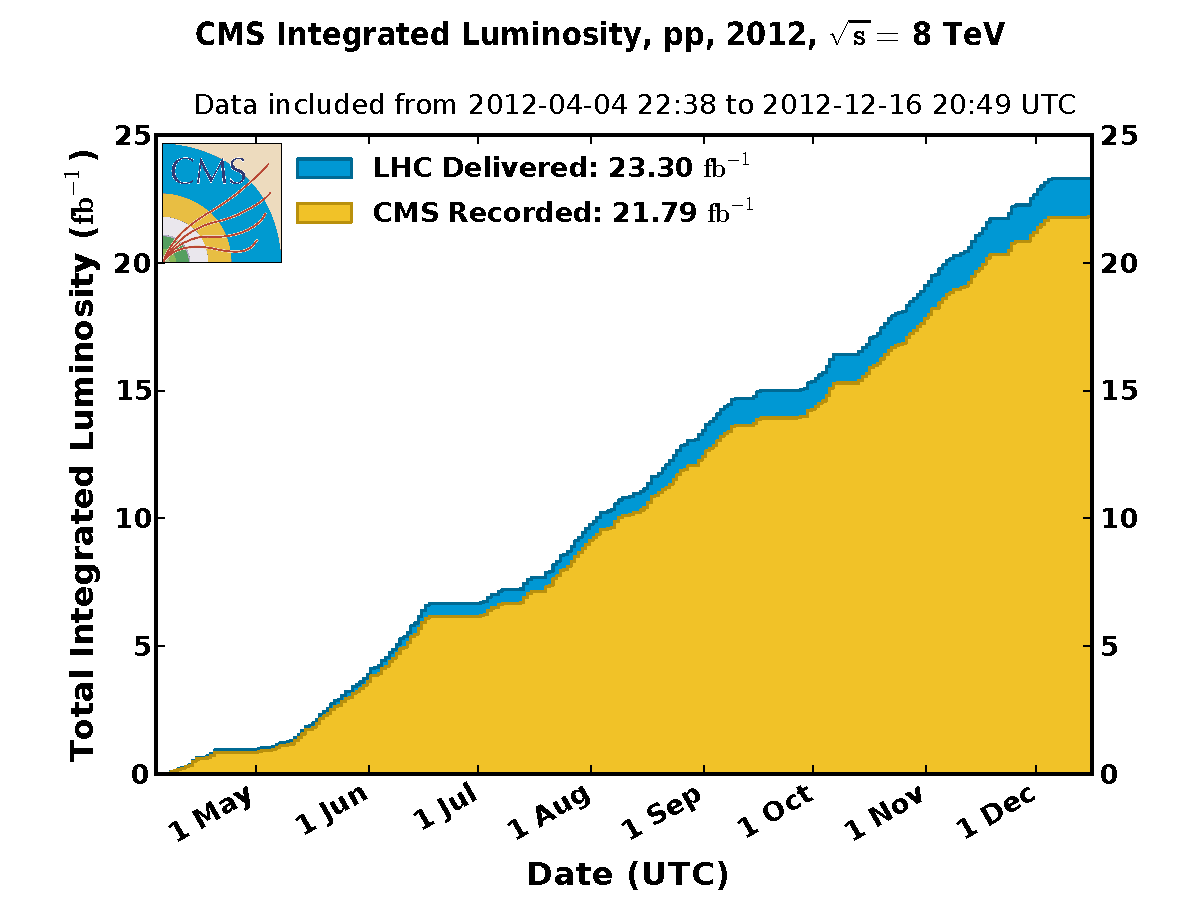
\includegraphics[width=0.55\textwidth]{figures/experiment/LHC/int_lumi_per_day_cumulative_pp_2012.pdf}
  \caption{Integrated luminosity delivered by LHC (blue) and recorded by CMS (orange) in the year 2012. Taken from~\cite{bib:LumiWiki}.}  
  \label{fig:Lumi}
\end{figure}

%%%%%%%%%%%%%%%%%%%%%%%%%%%%%%%%%%%%%%%%%%%%%%%%%%%%%%%%%%%%%%%%%%%%%%%%%%%%%%%%%%%%%%%%%%%%%%%%%%%%%%%%%%%%%%%%%%%%%%%%%%%%%%%%%%%%%%%%%%%%%%%%%%%%%%%%%%%%%%%%%%%%%%%%%%%%%%%%%%%%%%%%%%%%%%%%%%%%%%%%%%%%%%%%%%%%%%%%%%%%%%%%%%%
%%%%%%%%%%%%%%%%%%%%%%%%%%%%%%%%%%%%%%%%%%%%%%%%%%%%%%%%%%%%%%%%%%%%%%%%%%%%%%%%%%%%%%%%%%%%%%%%%%%%%%%%%%%%%%%%%%%%%%%%%%%%%%%%%%%%%%%%%%%%%%%%%%%%%%%%%%%%%%%%%%%%%%%%%%%%%%%%%%%%%%%%%%%%%%%%%%%%%%%%%%%%%%%%%%%%%%%%%%%%%%%%%%%
%%%%%%%%%%%%%%%%%%%%%%%%%%%%%%%%%%%%%%%%%%%%%%%%%%%%%%%%%%%%%%%%%%%%%%%%%%%%%%%%%%%%%%%%%%%%%%%%%%%%%%%%%%%%%%%%%%%%%%%%%%%%%%%%%%%%%%%%%%%%%%%%%%%%%%%%%%%%%%%%%%%%%%%%%%%%%%%%%%%%%%%%%%%%%%%%%%%%%%%%%%%%%%%%%%%%%%%%%%%%%%%%%%%
\FloatBarrier
\chapter{The CMS detector}
The Compact Muon Solenoid (CMS) detector~\cite{bib:CMS:experiment,bib:CMS:TDR} is a general purpose detector, designed to explore particle physics phenomena up to the multi-TeV scale.
The detector concept is an onion-like structure of different layers, each one made up of a different type of detector. 
The CMS detector measures 21.6\m in length and 14.6\m in diameter with a total weight of 12\,500\,tons.
In Fig.~\ref{fig:CMSdetector}, a perspective view of the CMS detector is depicted. 
\begin{figure}[!b]
  \centering
      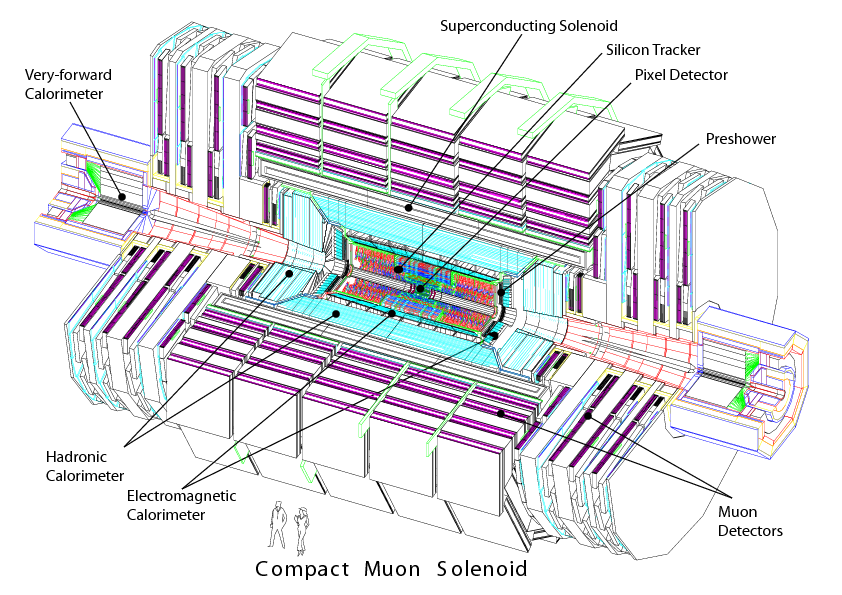
\includegraphics[width=0.89\textwidth]{figures/experiment/CMS/cms_complete_labelled.png}
  \caption{A perspective view of the CMS detector. Taken from~\cite{bib:CMS:experiment}}  
  \label{fig:CMSdetector}
\end{figure}

The coordinate system used at CMS consists of the pseudorapidity $\eta = -\ln \tan{\frac{\theta}{2}}$ and the azimuthal angle $\phi$.
The advantage of the pseudorapidity $\eta$ is the Lorentz invariance with respect to the z-axis (beam axis).
The angle $\phi$ covers the direction in the $x-y$ plane (orthogonal to the beam axis).

In order to measure the momentum of charged particles a superconducting solenoid is incorporated between the calorimeter system and the muon system providing a uniform axial magnet field of 3.8\tesla.
Iron yokes contained within the muon system ensure the return of the magnetic flux. 

In the following, the various detector components of the CMS detector from the inside to the outside as well as the trigger system will be explained.
%%%%%%%%%%%%%%%%%%%%%%%%%%%%%%%%%%%%%%%%%%%%%%%%%%%%%%%%%%%%%%%%%%%%%%%%%%%%%%%%%%%%%%%%%%%%%%%%%%%%%%%%%%%%%%%%%%%%%%%%%%%%%%%%%%%%%%%%%%%%%%%%%%%%%%%%%%%%%%%%%%%%%%%%%%%%%%%%%%%%%%%%%%%%%%%%%%%%%%%%%%%%%%%%%%%%%%%%%%%%%%%%%%%
\FloatBarrier
\section{The tracking system}
The tracking detector~\cite{bib:CMS:TDR_2006,bib:CMS:Tracker_1997,bib:CMS:Tracker_2000} is the innermost detector at CMS. 
It is a silicon semiconductor detector and is included for the tasks of vertex and track reconstruction by the measurement of particles' energy losses.
A schematic sketch of the tracker at CMS is depicted in Fig.~\ref{fig:Tracker}.
\begin{figure}[!b]
  \centering
      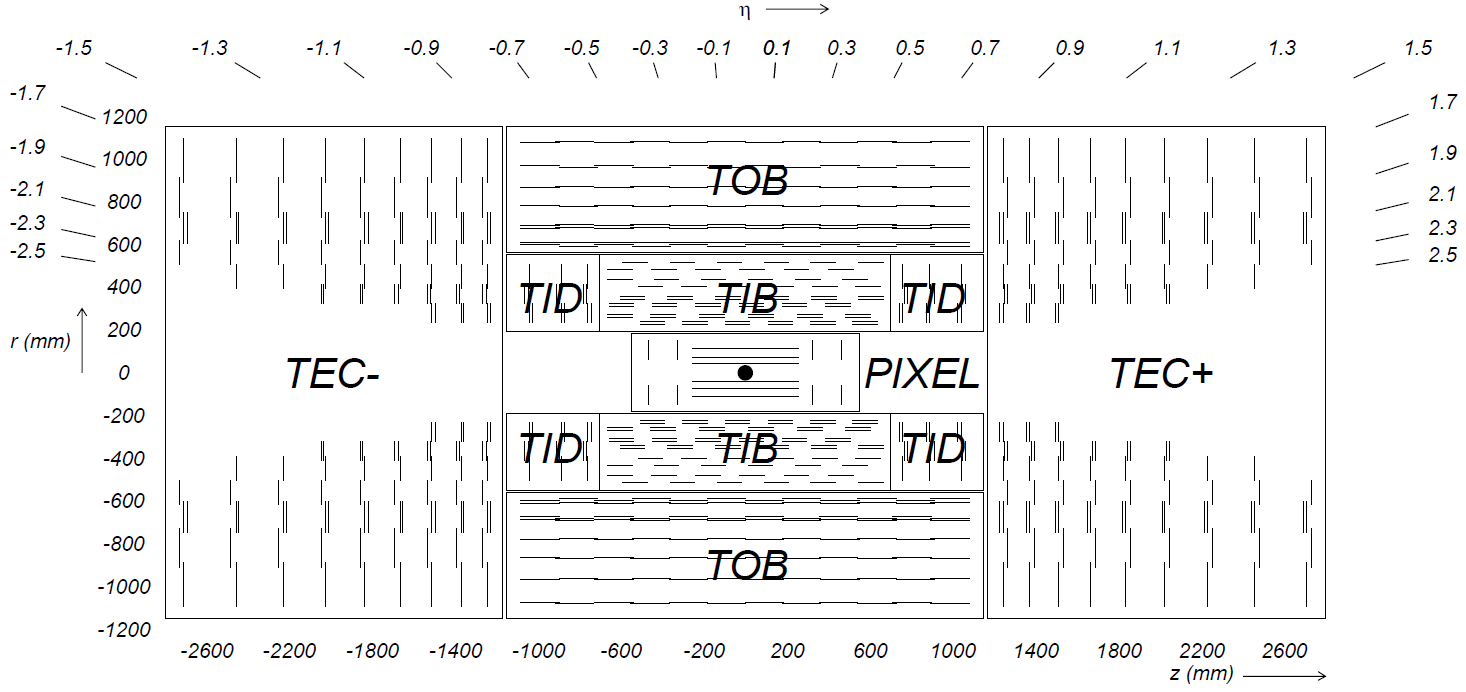
\includegraphics[width=0.99\textwidth]{figures/experiment/CMS/Figures_Experimental_Apparatus_Tracker.png}
  \caption{Schematic sketch of the silicon tracker at CMS in the $z - \phi$ plane including the silicon pixel detector (PIXEL) as well as the different components of the silicon strip detector: tracker inner barrel (TIB), tracker outer barrel (TOB), tracker endcap (TEC), and tracker inner disk (TID). Taken from~\cite{bib:CMS:tracking_8TeV}.
           }  
  \label{fig:Tracker}
\end{figure}
The tracking system is divided into two parts: the innermost tracker is a silicon pixel detector surrounded by a silicon strip detector.
Both parts will be explained in detail in the upcoming sections, followed by a short description of how the energy of a traversing particle is measured with the silicon sensors.
As a calibration of the silicon pixel detector was performed within this PhD thesis (see Section~\ref{sec:EnergyCalibration}), an emphasis will be put on the pixel detector.


%%%%%%%%%%%%%%%%%%%%%%%%%%%%%%%%%%%%%%%%%%%%%%%%%%%%%%%%%%%%%%%%%%%%%%%%%%%%%%%%%%%%%%%%%%%%%%%%%%%%%%%%%%%%%%%%%%%%%%%%%%%%%%%%%%%%%%%%%%%%%%%%%%%%%%%%%%%%%%%%%%%%%%%%%%%%%%%%%%%%%%%%%%%%%%%%%%%%%%%%%%%%%%%%%%%%%%%%%%%%%%%%%%%
\subsection*{The silicon pixel tracker}
The silicon pixel detector consists of three different cylindrical layers in the barrel region at radii of 4.4\cm, 7.3\cm and 10.2\cm and two discs in the endcaps at $z$-distances of 34.5\cm and 46.5\cm.
It is made up of 1440 modules in total (barrel + endcaps), each module comprising 8 or 16 read-out-chips (ROCs).
The read-out-chips are bump bonded~\cite{Thesis_Jenny} to a pixel system of $52\times80$ pixels, which are read out in double columns (see~\cite{Thesis_Jenny} on detailed information of the readout electronics).
A visualisation of a part of a pixel module is shown in Fig.~\ref{fig:PixelTracker}.
\begin{figure}[!b]
  \centering
      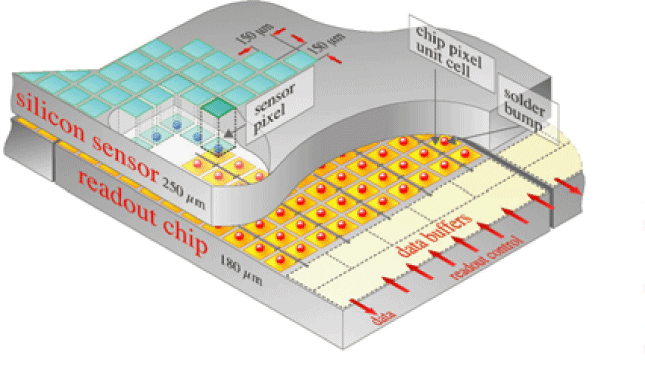
\includegraphics[width=0.90\textwidth]{figures/experiment/CMS/Pixelement.png}
  \caption{Schematic sketch of a part of a silicon pixel tracker module including the silicon sensors and the read-out-chip (ROC). Taken from~\cite{bib:CMS:tracking_8TeV}.}  
  \label{fig:PixelTracker}
\end{figure}
In total, there are 65 million pixels comprised in the pixel detector.
The large number of pixels and their small size ensure a low occupancy close to the vertex of around $0.002 - 0.02$\%~\cite{bib:CMS:tracking_8TeV} and a high hit efficiency of around 99\%~\cite{bib:CMS:PixelSpatialResolution}. 

The silicon pixel detector is very important for the reconstruction of primary and secondary vertices as well as the reconstruction of particle tracks.
Therefore, a high spatial resolution is needed.
This is achieved by the small size of the pixels ($ 150 \times 100 \mum^2$) and the exploitation of the spread of the energy deposition across several pixels (in average the energy is deposited across 3-5 pixels~\cite{bib:TWIKI:PixelClusterSize}).
Exploiting the energy spread across pixels, a spatial resolution in the barrel region of 9.4\mum in the $r - \phi$ plane and - dependent on the incident angle of a track - a hit resolution between $20-45\mum$ in the z-direction is achieved~\cite{bib:CMS:tracking_8TeV}. 
%The high spatial resolution makes the pixel detector perfectly suited for the reconstruction of vertices and tracks.
The spatial resolution of the primary vertex depends on the number of tracks taken into account for the reconstruction of the primary vertex.
For more than 50 tracks originating from the primary vertex the spatial resolution is around $10-12\mum$ for each of the three spatial dimensions~\cite{bib:CMS:tracking_8TeV}.
The reconstruction efficiency of primary vertices is close to 100\% if more than two tracks are used for the vertex reconstruction~\cite{bib:CMS:tracking_8TeV}.

\subsection*{The silicon strip tracker}
The silicon strip tracker is the next-to innermost detector of the CMS detector and ranges up to a radius of 1.1\m.
The barrel region consists of a tracker inner barrel (TIB) and a tracker outer barrel (TOB).
The TIB has four layers with two layers equipped with stereo modules to measure the hit position additionally in the $r-z$ plane.
The silicon sensors in the TIB are of 320\mum thickness with a strip pitch varying between $80-120\mum$.
The TOB has six different layers (two layers of stereo modules) with silicon sensors of 500\mum thickness and strip pitches between 120 and 180\mum. 

The endcaps are subdivided into a tracker endcap (TEC) and a tracker inner disk (TID).
They ensure a coverage of a pseudorapidity up to $|\eta|=2.5$.
In each TEC, 9 disks between a z-position of $120\cm < z < 280\cm$ are contained.
Each of the TID comprises three disks between $60\cm < z < 110\cm$.

In the barrel region, a single-point resolution between $23 - 52\mum$ in the $r-\phi$ plane and $230 - 530\mum$  in the z-direction is achieved.
%FIXME: What about momentum resolution

\subsection*{Energy measurements in the tracking system}
A charged particle traversing the above mentioned silicon detectors produces electron-hole pairs in the semiconducting material along its trajectory, thus loosing energy due to ionisation.
For silicon, the mean energy to create an electron-hole pair is 3.61\ev at $-10\degree$C.
Minimally ionising particles produce an average of 22\,000 electron-hole pairs in silicon sensors~\cite{Thesis_Jenny}.
Electrons that are subject to a hard collision with the incoming particle (so-called delta-rays), produce further ionisation and can thus lead to much higher energy deposits in the silicon.
Because of the applied bias voltage at the sensors (for the creation of a depletion zone), the released electrons (holes) travel to the n-contacts (p-contacts), thereby inducing a current which is measured by the readout electronics. 
A more detailed description of the energy measurement in silicon sensors can be found in~\cite{Thesis_Jenny}.

%%%%%%%%%%%%%%%%%%%%%%%%%%%%%%%%%%%%%%%%%%%%%%%%%%%%%%%%%%%%%%%%%%%%%%%%%%%%%%%%%%%%%%%%%%%%%%%%%%%%%%%%%%%%%%%%%%%%%%%%%%%%%%%%%%%%%%%%%%%%%%%%%%%%%%%%%%%%%%%%%%%%%%%%%%%%%%%%%%%%%%%%%%%%%%%%%%%%%%%%%%%%%%%%%%%%%%%%%%%%%%%%%%%
\section{The electromagnetic calorimeter}
The electromagnetic calorimeter (ECAL)~\cite{bib:CMS:TDR_2006,bib:CMS:TDR_ECAL} encloses the tracking system and starts at a radius of 129\cm in the barrel region.
It is divided into a barrel part and two endcaps, which are at a distance of 314\cm from the vertex.
Figure~\ref{fig:ECAL} depicts a schematic sketch of the electromagnetic calorimeter system in the transverse plane.
\begin{figure}[!ht]
  \centering
      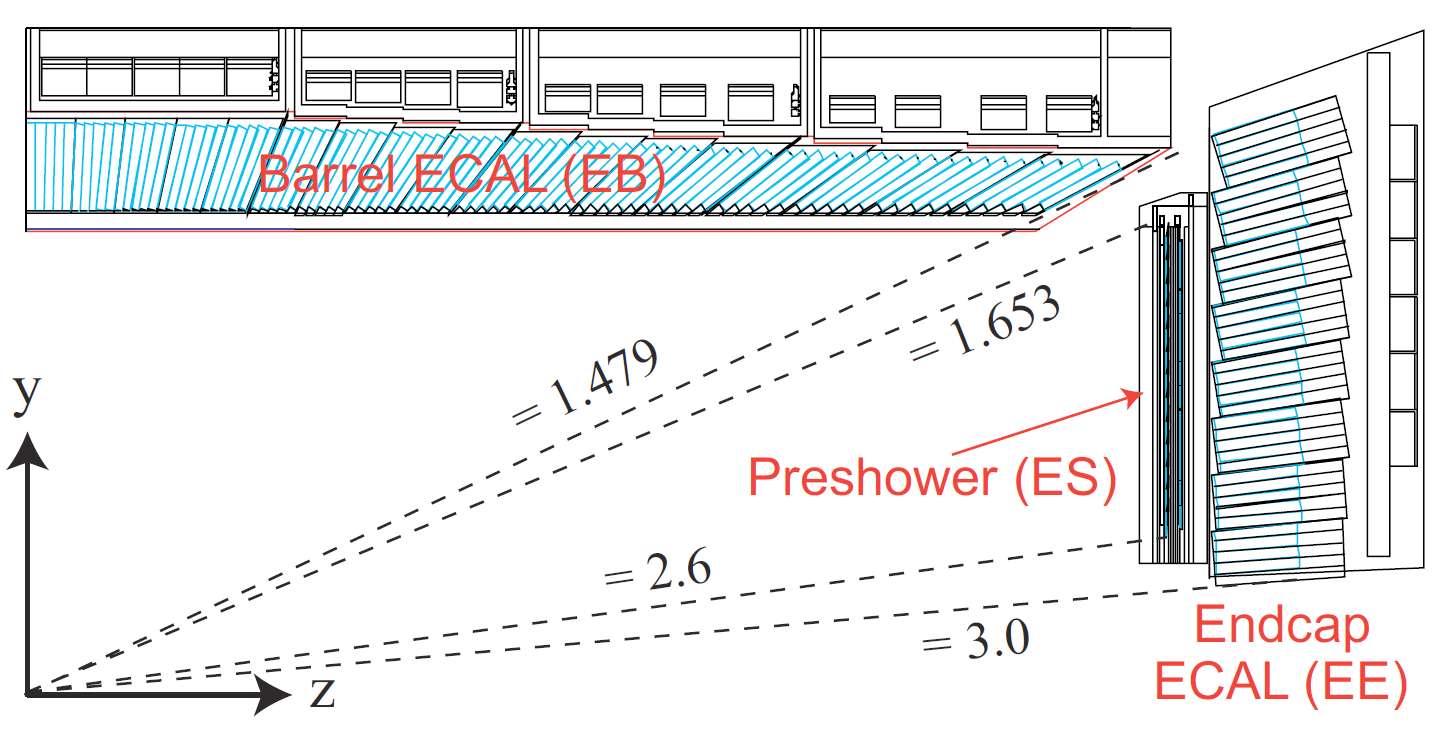
\includegraphics[width=0.89\textwidth]{figures/experiment/CMS/Figures_Experimental_Apparatus_ECALRapidity.png}
  \caption{A quarter section of the ECAL in a transverse view. Taken from~\cite{bib:CMS:TDR_2006}.}  
  \label{fig:ECAL}
\end{figure}
It can be seen, that the ECAL barrel~(EB) covers a pseudorapidity region up to $|\eta|=1.479$.
The ECAL endcaps~(EE) start at $|\eta|=1.653$ and reach up to $|\eta|=3.0$.
Before the endcaps, a preshower detector ($1.653<|\eta|<2.6$) is installed with the main task to identify neutral pions in the endcaps.
It additionally improves the position measurement of electrons and photons.

The EB and EE consist of lead tungstate (PbWO$_4$) scintillating crystals, 61200 in the barrel region and 7324 in the endcaps. 
Their advantage is the short radiation length (X$_0$=0.89\cm) and a small Moli\`ere radius (2.2\cm).
Thus, particles deposit their energy on rather short distances and a compact design is possible.
To detect the rather low light yield (30$\gamma$/\mev) of a traversing particle, silicon avalanche photodiodes (APDs) are used in the barrel region and vacuum  phototriodes (VPTs) in the endcaps.
For information on the readout electronics, the reader is referred to~\cite{bib:CMS:TDR_2006}.

The resolution of an energy measurement in the calorimeter can be expressed by 
\begin{equation}
\label{eq:CaloResolution}
\left( \frac{\sigma}{E} \right)^2 = \left( \frac{S}{\sqrt{E}} \right)^2 + \left( \frac{N}{E} \right)^2 +C^2,
\end{equation}
with $S$ referring to the stochastic term, $N$ to the noise term, and $C$ to a constant term.
For the ECAL the parameters of Eq.~\eqref{eq:CaloResolution} are measured to $S=3.63\sqrt{\text{GeV}}$, $N=0.124\gev$, and $C=0.26$~\cite{bib:CMS:TDR_2006}. 
These numbers lead to an energy resolution of around 0.4\% for an electron with $E \approx 200\gev$ and around 0.6\% for an electron with $E \approx 50\gev$.

%%%%%%%%%%%%%%%%%%%%%%%%%%%%%%%%%%%%%%%%%%%%%%%%%%%%%%%%%%%%%%%%%%%%%%%%%%%%%%%%%%%%%%%%%%%%%%%%%%%%%%%%%%%%%%%%%%%%%%%%%%%%%%%%%%%%%%%%%%%%%%%%%%%%%%%%%%%%%%%%%%%%%%%%%%%%%%%%%%%%%%%%%%%%%%%%%%%%%%%%%%%%%%%%%%%%%%%%%%%%%%%%%%
\section{The hadronic calorimeter}
The hadronic calorimeter (HCAL)~\cite{bib:CMS:TDR_2006,bib:CMS:TDR_HCAL} of the CMS detector is splitted into four different detector modules: the hadron barrel (HB), the hadron outer (HO), the hadron endcap (HE) and the hadron forward (HF) calorimeters.
A schematic sketch is depicted in Fig.~\ref{fig:HCAL}.
\begin{figure}[!ht]
  \centering
      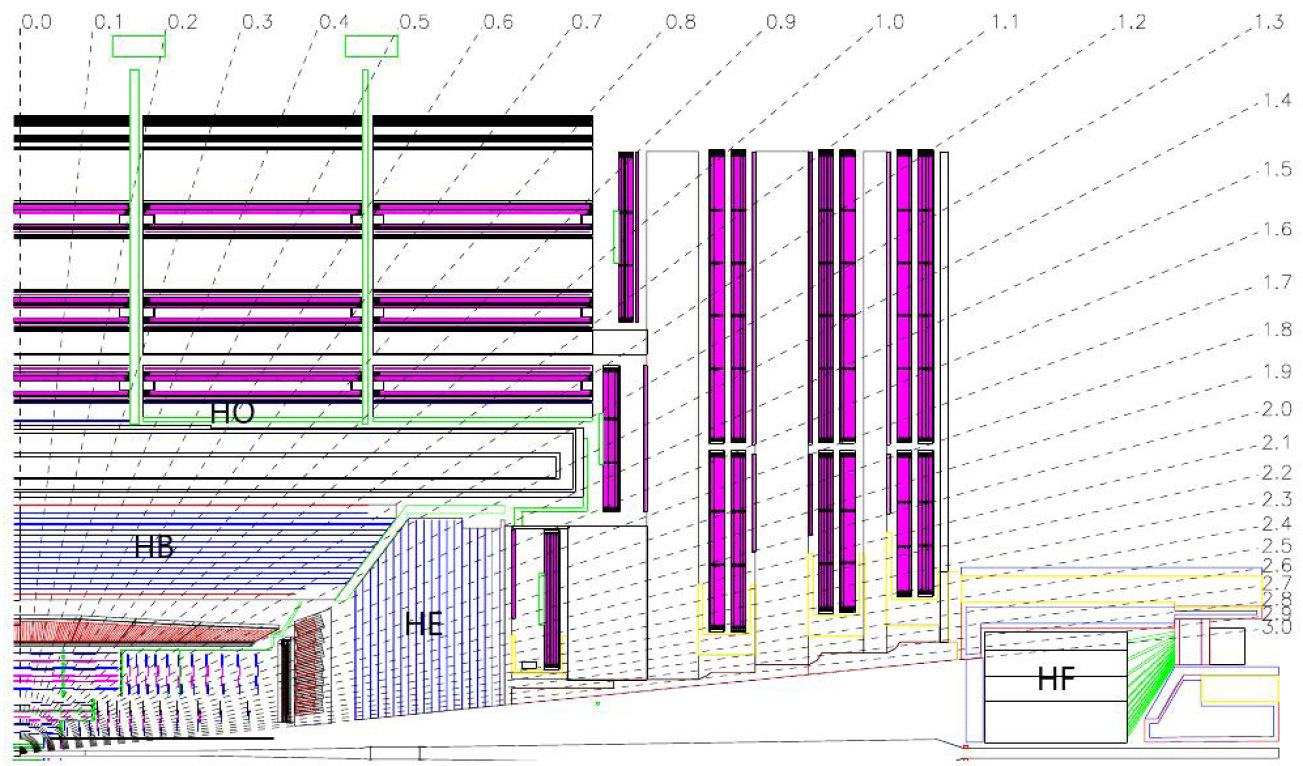
\includegraphics[width=0.79\textwidth]{figures/experiment/CMS/fig_HCALdiagram.png}
  \caption{A quarter section of the HCAL in a transverse view. Taken from~\cite{bib:CMS:HCAL_Performance_2009}.}  
  \label{fig:HCAL}
\end{figure}

The HCAL is dedicated to measuring the energy of hadrons as well as providing a good estimate of the missing energy in the event.
The latter one is achieved by the high pseudorapidity coverage ($|\eta|<5.0$) that assures the detection of most of the visible particles.

The HCAL is a so-called sampling calorimeter which consists of brass absorber material, initiating the hadronic shower, as well as active plastic scintillators.
The emitted photons are read out with wavelength-shifting (WLS) fibres which are embedded into the scintillators.
These in turn are connected to clear fibres that transfer the light to the readout system.

The hadron barrel (HB) covers the pseudorapidity range between $-1.4 < \eta < 1.4$.
It is composed of 17 layers of absorber material (15 brass and 2 steel layers) interleaved with scintillator layers.
The scintillator layers are divided into 2304 towers with a size of $\Delta \eta \times \Delta \phi = 0.087 \times 0.087$.

The hadron outer (HO) covers a pseudorapidity range up to $|\eta|=1.26$ and is divided into sectors which match the $\phi$ segmentation of the drift-tube chambers of the muon system (see Section~\ref{sec:MuonSystem}).
It is located between the solenoid and the barrel detector of the muon system.
The HO is dedicated to measuring the energy of the shower leakage of hadrons.
Its thickness corresponds to over ten interaction lengths.

The hadron endcap (HE) extends the pseudorapidity coverage of the HCAL up to $|\eta|=3.0$ and starts at $|\eta|=1.3$.
It consists of 2304 towers in total, which vary in size between $5-10\degree$ in the $\phi$ direction and $0.087-0.35$ in $\eta$ direction.

Finally, the hadron forward (HF) calorimeter extends the pseudorapidity range up to $|\eta|=5.0$, starting from $|\eta|=3.0$.
It is build out of steel plates, which contain $1\mm^2$ grooves containing quartz fibres.
The emitted light by the quartz fibres is transferred to photomultipliers.
The HF is divided into 13 towers where almost all towers have a spread of $\Delta \eta \approx 0.175$ in $\eta$ direction and $\sim 10\degree$ in $\phi$ direction.
 
%%%%%%%%%%%%%%%%%%%%%%%%%%%%%%%%%%%%%%%%%%%%%%%%%%%%%%%%%%%%%%%%%%%%%%%%%%%%%%%%%%%%%%%%%%%%%%%%%%%%%%%%%%%%%%%%%%%%%%%%%%%%%%%%%%%%%%%%%%%%%%%%%%%%%%%%%%%%%%%%%%%%%%%%%%%%%%%%%%%%%%%%%%%%%%%%%%%%%%%%%%%%%%%%%%%%%%%%%%%%%%%%%%
\section{The muon system}
\label{sec:MuonSystem}
The muon system~\cite{bib:CMS:TDR_2006,bib:CMS:TDR_MuonSystem} is the outermost detector component at CMS.
It comprises three different types of gaseous detectors, mounted into the iron return yokes: drift tube (DT) chambers in the barrel region ($|\eta|<1.2$), cathode strip chambers (CSC) in the endcap region ($1.04<|\eta|<2.4$) and resistive plate chambers (RPC) in the barrel as well as the endcap region ($|\eta|<1.6$) (see Fig.~\ref{fig:MuonSystem} for a schematic sketch of the muon system).
\begin{figure}[!b]
  \centering
      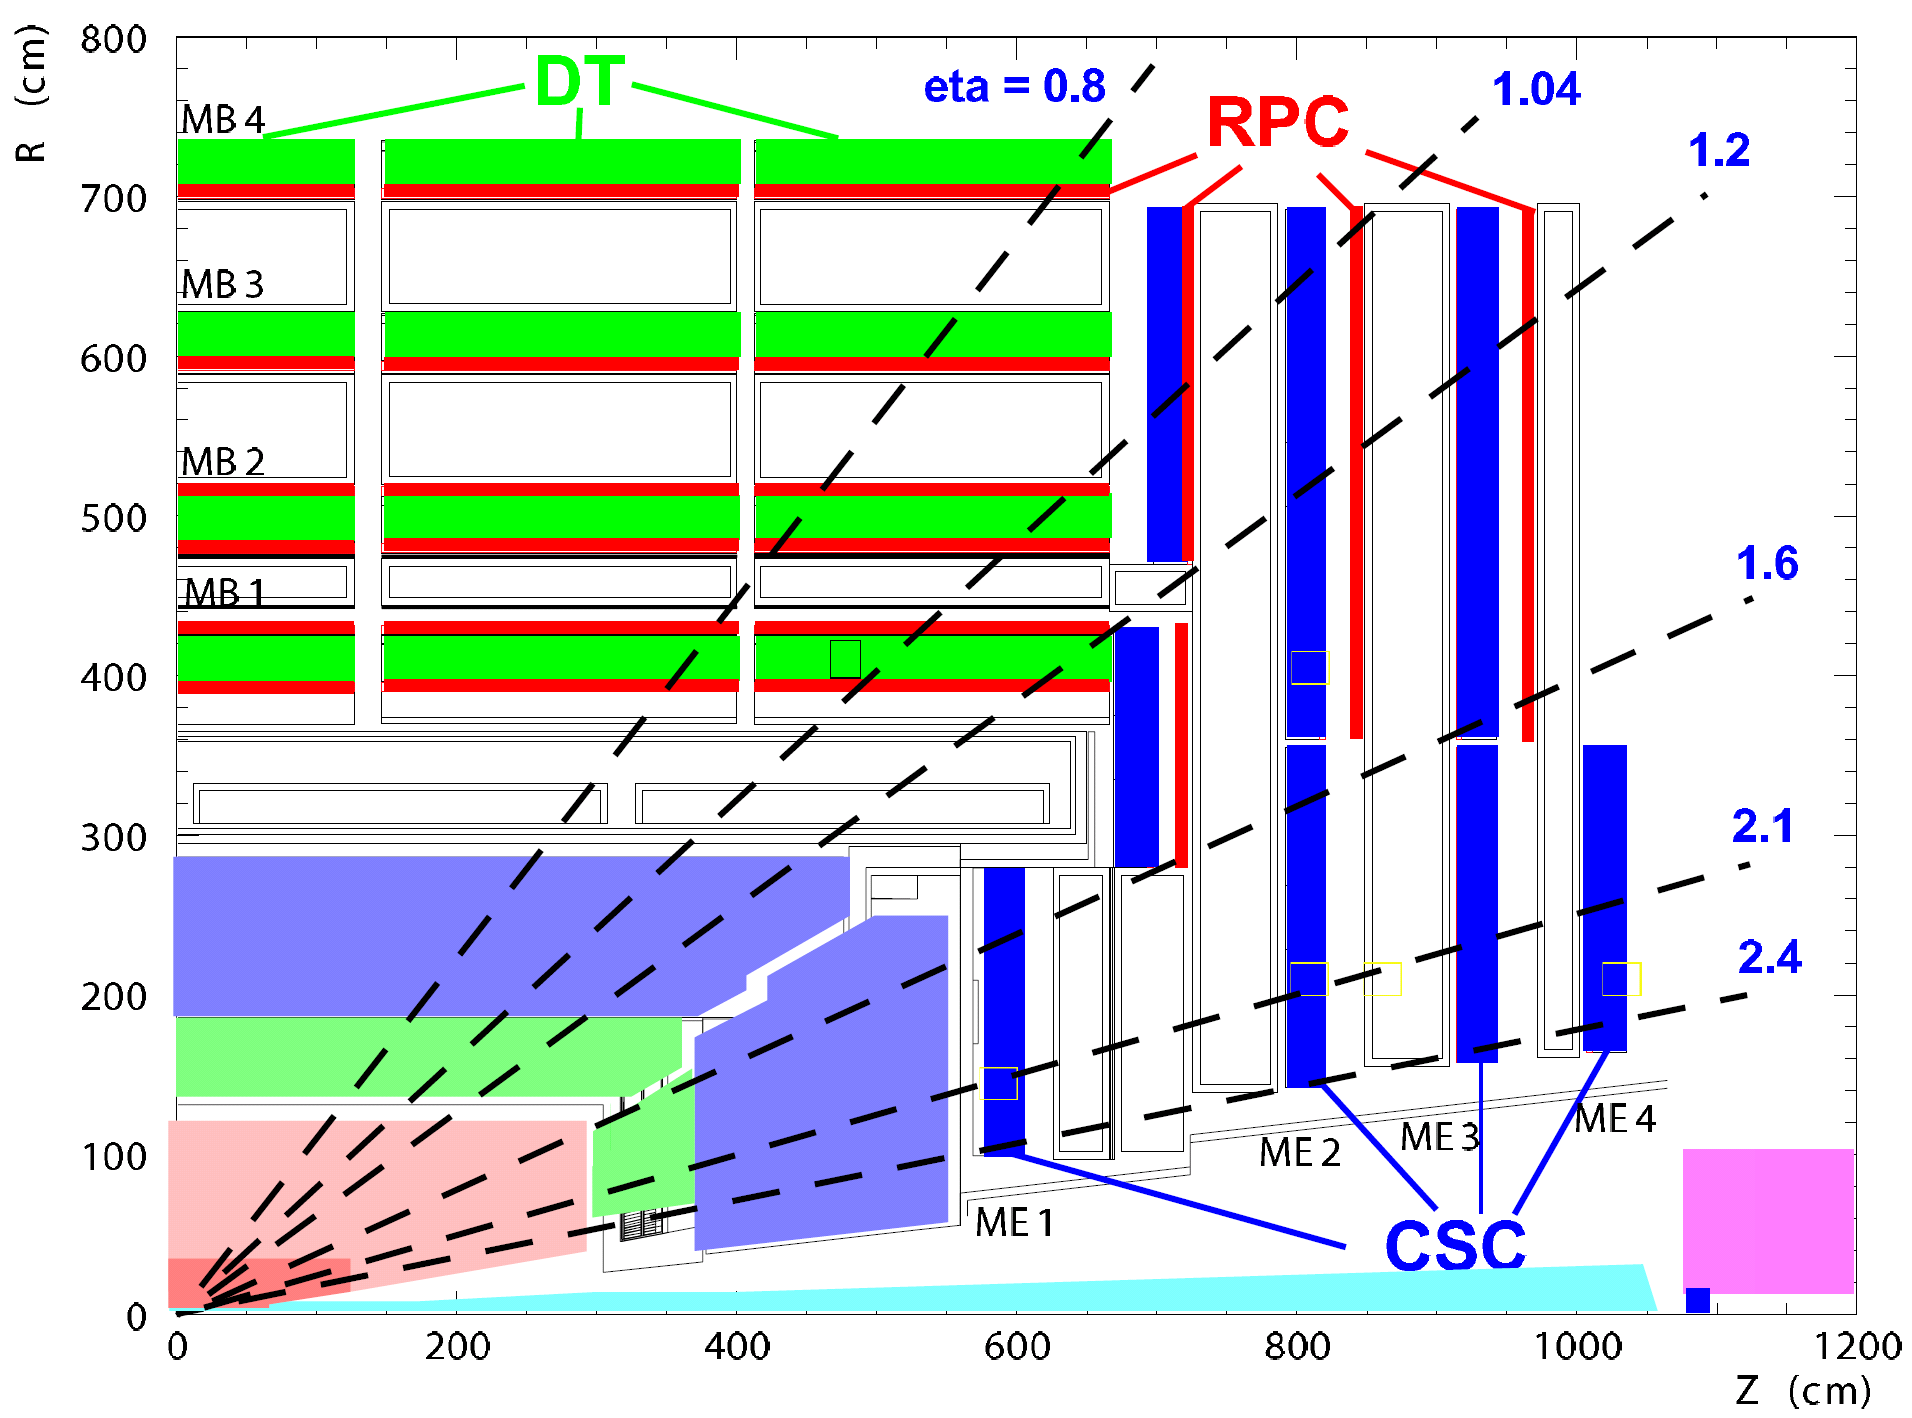
\includegraphics[width=0.69\textwidth]{figures/experiment/CMS/Figures_Experimental_Apparatus_MuonDetector.png}
  \caption{A quarter section of the CMS detector in the transverse plane with a detailed view on the muon system. Taken from~\cite{bib:CMS:TDR_2006}.}  
  \label{fig:MuonSystem}
\end{figure}
In the barrel part of the muon system, four layers (so-called stations) of drift-tube chambers are assembled inside the iron return yoke layers at radii of 4.0, 4.9, 5.9 and 7.0\m from the beam axis.
The position of a muon traversing these layers can be measured with a precision of $\approx 100\mum$ in radial direction and $\approx 1\,$mrad in $\phi$ direction. 

The four endcap disks are made up of 468 cathode strip chambers in total.
By measuring the centre-of-gravity, they achieve a spatial resolution of $\approx 100-200\mum$ and an angular resolution of $\approx 10\,$mrad in $\phi$ direction.
They are designed in order to cope with a high particle flux of about 1kHz/cm$^2$ and a non-uniform magnetic field.
As signals can be transferred very fast, they are used for the level-1 trigger system.

Finally, the resistive plate chambers cover the barrel as well as the endcap region up to a pseudorapidity of $\eta=1.6$. 
They provide a fast response with a good time resolution enabling the exact identification of the respective bunch-crossing.
It is used for the level-1 trigger system as well.
%%%%%%%%%%%%%%%%%%%%%%%%%%%%%%%%%%%%%%%%%%%%%%%%%%%%%%%%%%%%%%%%%%%%%%%%%%%%%%%%%%%%%%%%%%%%%%%%%%%%%%%%%%%%%%%%%%%%%%%%%%%%%%%%%%%%%%%%%%%%%%%%%%%%%%%%%%%%%%%%%%%%%%%%%%%%%%%%%%%%%%%%%%%%%%%%%%%%%%%%%%%%%%%%%%%%%%%%%%%%%%%%%%
\section{The trigger system}
Because of the impossibility of storing each event occurring at the CMS experiment, a multistage trigger system~\cite{bib:CMS:TDR_2006} is used to achieve a drastic reduction of recorded events by nearly six orders of magnitude.
It comprises two main parts: a so-called level-1 (L1) trigger system and a high-level trigger (HLT) system.

The L1 triggers need to provide a very fast decision (3.2\mus, where around 1\mus is allocated to the actual L1 trigger calculations) whether an event shall be recorded or not.
During this time, the recorded event data is held in buffers located close to the single detector components.
Information from the muon system and the calorimeters is used for the L1-trigger decisions.
Objects used for these decisions are so-called ``trigger primitive'' objects: photons, electrons, muons, jets above certain \et and \pt thresholds and global variables like missing transverse energy, \met. 
The design value of the number of events per second that pass this trigger stage is 100\khz.

After a time of 3.2\mus, the stored data in the buffers close to the single detector components are transferred to the front-end readout buffers in case the event passed the L1-trigger requirements.
By partial event reconstruction and the use of various trigger levels (calorimeter, muon information followed by pixel information and full event reconstruction), higher event objects can be used to check whether HLT-trigger requirements are fulfilled.
On HLT level, the decision time amounts to 50\ms and a reduction from 100\khz to 100\hz of event recording is achieved.

%%%%%%%%%%%%%%%%%%%%%%%%%%%%%%%%%%%%%%%%%%%%%%%%%%%%%%%%%%%%%%%%%%%%%%%%%%%%%%%%%%%%%%%%%%%%%%%%%%%%%%%%%%%%%%%%%%%%%%%%%%%%%%%%%%%%%%%%%%%%%%%%%%%%%%%%%%%%%%%%%%%%%%%%%%%%%%%%%%%%%%%%%%%%%%%%%%%%%%%%%%%%%%%%%%%%%%%%%%%%%%%%%%%
%%%%%%%%%%%%%%%%%%%%%%%%%%%%%%%%%%%%%%%%%%%%%%%%%%%%%%%%%%%%%%%%%%%%%%%%%%%%%%%%%%%%%%%%%%%%%%%%%%%%%%%%%%%%%%%%%%%%%%%%%%%%%%%%%%%%%%%%%%%%%%%%%%%%%%%%%%%%%%%%%%%%%%%%%%%%%%%%%%%%%%%%%%%%%%%%%%%%%%%%%%%%%%%%%%%%%%%%%%%%%%%%%%%
%%%%%%%%%%%%%%%%%%%%%%%%%%%%%%%%%%%%%%%%%%%%%%%%%%%%%%%%%%%%%%%%%%%%%%%%%%%%%%%%%%%%%%%%%%%%%%%%%%%%%%%%%%%%%%%%%%%%%%%%%%%%%%%%%%%%%%%%%%%%%%%%%%%%%%%%%%%%%%%%%%%%%%%%%%%%%%%%%%%%%%%%%%%%%%%%%%%%%%%%%%%%%%%%%%%%%%%%%%%%%%%%%%%
\FloatBarrier
\chapter{Event reconstruction and particle identification}
A crucial ingredient of data analysis at the CMS experiment, is the translation of the energy measurements in the various sub-detector components into physical objects, like muons, electrons, \etc.
For this translation, \ie particle identification, information from all detector components are used.
This is know as the particle-flow event reconstruction algorithm~\cite{CMS-PAS-PFT-09-001}.
In Fig.~\ref{fig:CMSslice}, a slice through the CMS detector is shown with the signatures of different particles indicated as coloured lines.

In the next section an introduction into this algorithm is given, followed by the definition and classification of physics objects at the CMS experiment.

\begin{figure}[!ht]
  \centering
      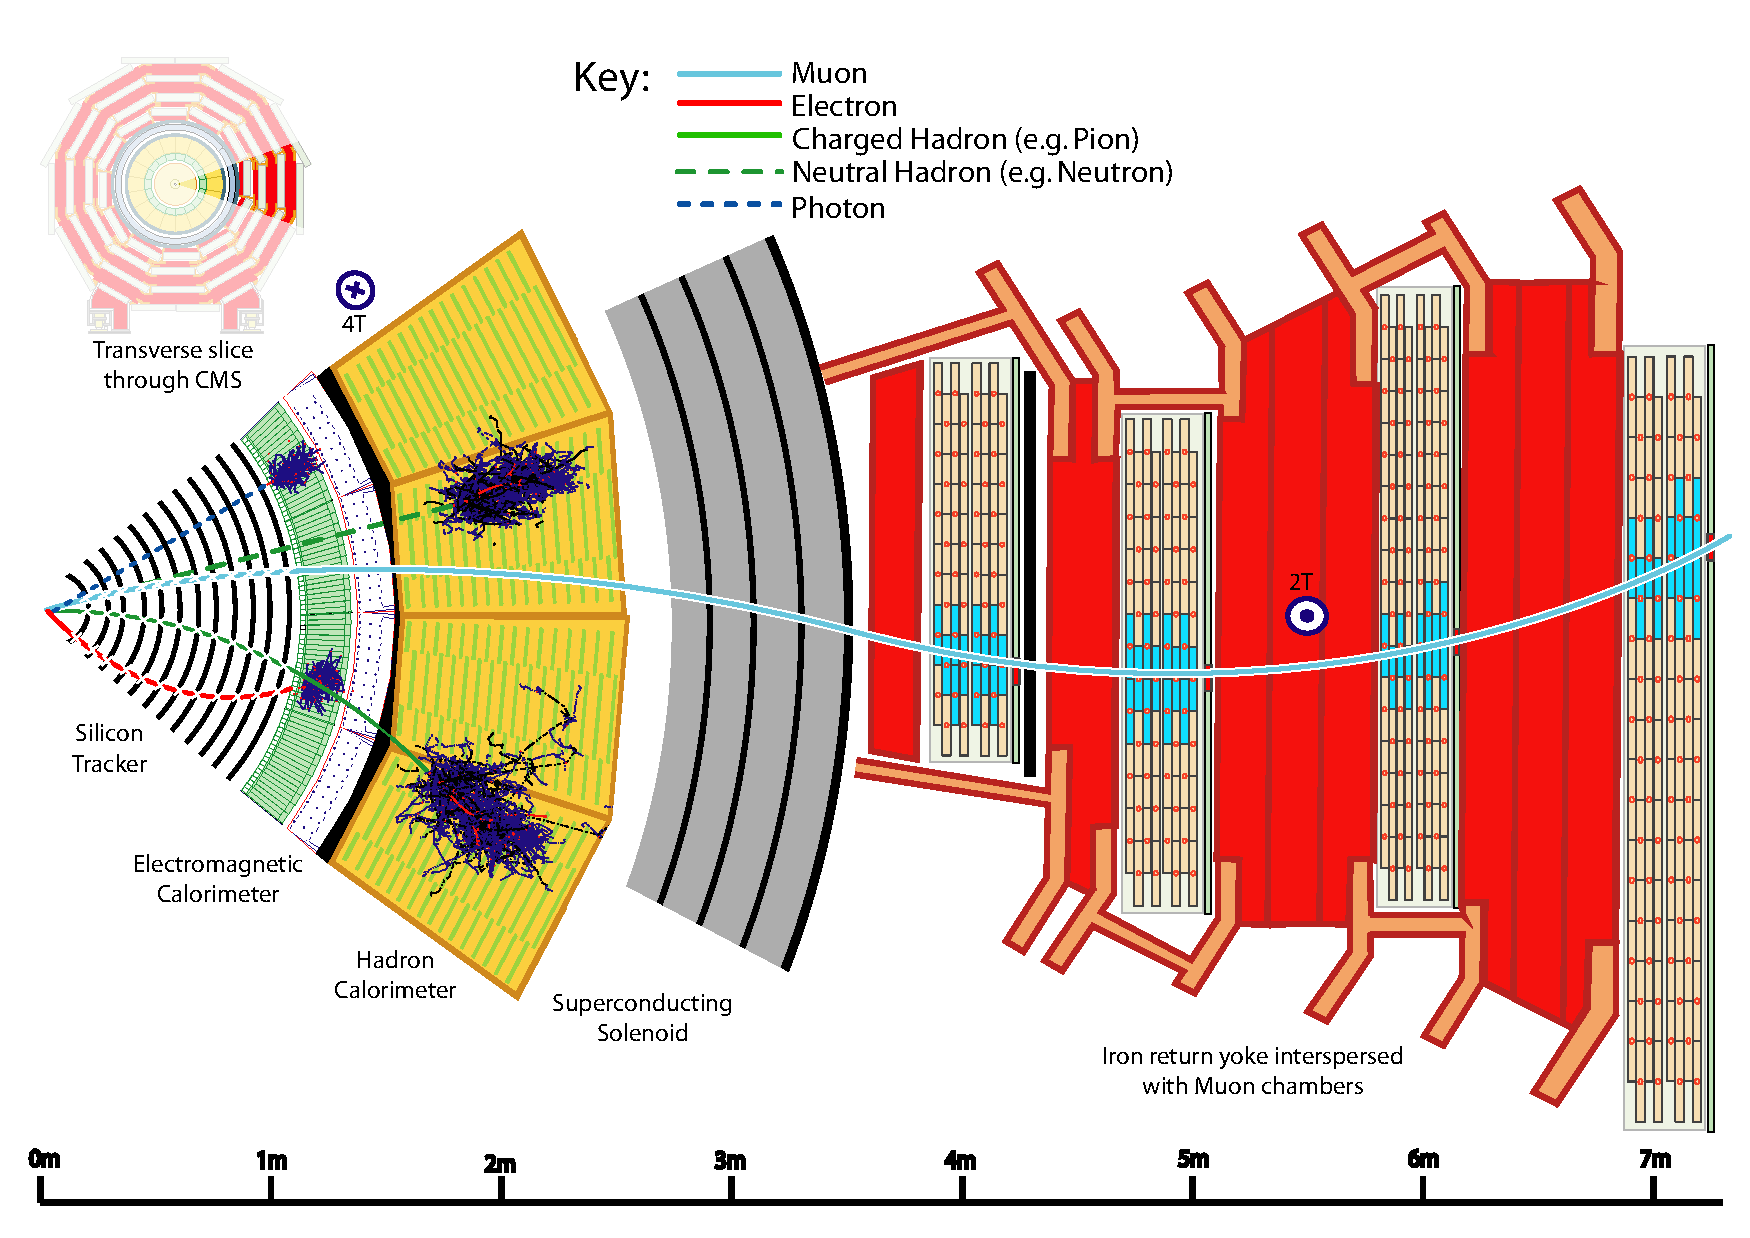
\includegraphics[width=0.99\textwidth]{figures/experiment/ObjectReconstruction/slice_white.pdf}
  \caption{A radial slice through the CMS detector with several particle signatures indicated as coloured lines.}  
  \label{fig:CMSslice}
\end{figure}

%This is done by defining what kind of energy deposits are necessary in order to classify signals during an event as a muon, \etc.
%For this classification, a certain catalogue is set up, which specifies when to classify energy signals as a certain particle.

\section{The particle-flow algorithm}
\label{sec:PFalgorithm}
The particle-flow (PF) event description~\cite{CMS-PAS-PFT-09-001} aims at optimising particle identification by the usage of all sub-detector components of the CMS detector.
There are three main building bricks used for the global event description: reconstructed charged-particle tracks, calorimeter clusters, and muon tracks.
The main requirements for these building bricks is a high reconstruction efficiency as well as a small fake rate.
Therefore, a special emphasis was put on developing a very efficient tracking algorithm (see Section~\ref{sec:ObjectReconstruction}) and a well performing calorimeter clustering algorithm~\cite{CMS-PAS-PFT-09-001}. 

The particle-flow algorithm proceeds as follows in an event (the following steps are a bit simplistic, the reader is referred to~\cite{CMS-PAS-PFT-09-001} for a detailed discussion):
\begin{enumerate}
\item For each pair of detected building bricks, a distance in the $\eta-\phi$ plane is calculated in order to quantify the quality of their link (whether the two building bricks stem from the same particle). 
\item ``Blocks'' are produced from the building bricks that are linked together (with a typical number of one, two or three building bricks contained in a block).
\item For each block the following steps are performed:
\begin{enumerate}
\item Each global muon (hits detected in the tracker as well as in the muon system) where the \pt measured in both sub-detectors is compatible with the tracker measurement only is defined as particle-flow muon and the track in both sub-detectors is removed from the event.
\item Electron reconstruction and identification follows using blocks with tracker hits and ECAL clusters. 
      For an identified particle-flow electron, the corresponding tracker hits and the ECAL clusters (including energy deposits from Bremsstrahlung photons) are removed. 
\item Tighter tracker quality criteria are applied.
\item The compatibility of the remaining ECAL and HCAL energy deposits to transverse momentum of the reconstructed tracks within a block is checked. 
      This allows for the identification of particle-flow charged hadrons with a momentum estimate using tracker and calorimeter information. 
      Only, if the energy deposits in the ECAL or HCAL are much larger than the corresponding track \pt, it gives rise to a particle-flow photon or particle-flow neutral hadron. 
      All used ECAL and HCAL clusters used for the identification as well as the reconstructed tracks are removed from the event.
\item Finally, the remaining HCAL and ECAL clusters (which are all not linked to any other building block) give rise to particle-flow photons or particle-flow neutral hadrons.
\end{enumerate}
\end{enumerate}
These identified particle-flow objects are used to identify further objects in the event, \eg the missing transverse-energy or decay products of a tau lepton.

\section{Object reconstruction}
\label{sec:ObjectReconstruction}
In this section, an overview about the required criteria for the identification of particles and other physics object is given.
\subsection*{Reconstruction of tracks}
The reconstruction of tracks aims at linking several hits in the tracking system to one reconstructed track that matches with a high probability the original trajectory of the particle.
With the track reconstruction an estimate of the particle's momentum as well as the position can be achieved.
The challenge arise due to the high combinatorial complexity because of the large number of hits detected in each event, especially in the layers close to the interaction vertex.
In the following an overview about the tracking algorithm used at CMS is given.
The reader is referred to~\cite{bib:CMS:tracking_8TeV} for a thorough description of the reconstruction of tracks at CMS.

The developed tracking software used at CMS is usually referred to as the Combinatorial Track Finder (CTF).
It grounds on the so-called combinatorial Kalman filter~\cite{bib:TrackAlgorithm_1989,bib:TrackAlgorithm_1990,bib:TrackAlgorithm_1997}, which is mathematically equivalent to a global least square minimisation for linear models with Gaussian noise.

The basic idea of the tracking algorithm at CMS is to not apply the combinatorial Kalman filter on all hits in one step but to reduce the level of complexity by an iterative procedure (called iterative tracking).
A reduction of complexity can be achieved by reconstructing tracks in the first step that are easy to identify because of \eg a high \pt. 
These tracks are removed afterwards and the remaining tracker hits are subject to further reconstruction iterations.
%In the following, the various iteration steps are described.
%These were in place in the year 2011.
%Adjustment in the algorithm were applied due to higher pileup conditions in the year 2012.
%However, the principle structure of the tracking algorithm remained.
The following iterations are performed:
\begin{itemize}
\item Iteration 0: Tracks near to the $pp$ interaction point that have three pixel hits and a $\pt>0.8\gev$ are reconstructed.
\item Iteration 1: Tracks with only two pixel hits and $\pt>0.8\gev$ are recovered.
\item Iteration 2: Low \pt tracks from the $pp$ interaction point are reconstructed.
\item Iteration 3-5: Reconstruction of tracks that are not originating from the primary vertex and recovering of tracks not found by previous iterations
\end{itemize}
Within these iterations, the reconstruction is subdivided into four different steps:
\begin{itemize}
\item Seed generation: Only 2-3 hits are used to define track candidates.
\item Extrapolation: Based on expected flight path, additional hits are assigned to the candidate track (use of Kalman filter)
\item Parameter estimates: With the usage of the Kalman filter and a smoother the trajectory parameters are determined
\item Setting of quality flags: Quality flags are assigned to all tracks and tracks that fail certain quality criteria are discarded.
\end{itemize}
The configuration of the first and the fourth step differ across the different iterations.  

\subsection*{Reconstruction of jets} 
The reconstruction of jets is done by a anti-kt method at CMS.
\begin{itemize}
\item Clustering methods: anti kt method
\item jet energy corrections
\end{itemize}

\subsection{Reconstruction of muons}
There are three different muon definitions at CMS~\cite{bib:CMS:muon_recoEff}: global muons (correspond to particle-flow muons), tracker muons, and standalone muons.
They have all in common that they require energy deposits in the muon system.
The reconstruction of each of the three muon types is explained in the following.
\begin{description}
\item \textbf{Standalone muons:} For the reconstruction of standalone muons, all reconstructed segments in the muon system are utilised. Similar to the track reconstruction in the tracking system, Kalman filter techniques~\cite{bib:KalmanFilter_1987} are exploited to reconstruct muon trajectories in the muon chambers.
A compatibility to the interaction point is imposed to reconstruct only muons produced at the LHC (no cosmic muons).
Further details about the reconstruction of standalone muons can be found in~\cite{bib:StandaloneMuonReconstruction,bib:CMS:TDR_2006} 
\item \textbf{Tracker muons:} To reconstruct so-called tracker muons, all tracker tracks with a $\pt>0.5\gev$ and $p>2.5\gev$ are extrapolated to the muon system. If at least one muon segment is matched to a reconstructed track within certain quality criteria, the trajectory is considered as a tracker muon (see~\cite{bib:CMS:muon_recoEff} for more detailed information).
\item \textbf{Global muons:} For the reconstruction of global muons an outside-in approach is utilised. For each reconstructed standalone muon, the compatibility to the reconstructed tracks in the tracking system is checked. If compatible, a global muon track is reconstructed using Kalman filter techniques. For high-\pt muons, the momentum resolution can be increased compared to the momentum estimated using tracker information only~\cite{bib:CMS:muon_recoEff}.
\end{description}

\subsection{Reconstruction of electrons}
The reconstruction of electrons at the CMS experiment is based on a mixture of the particle-flow algorithm explained in Section~\ref{sec:PFalgorithm} and a standalone approach~\cite{bib:StandaloneElectronReconstruction}.
Thus, it is a very complex procedure and a complete description would go beyond the scope of this thesis.
Therefore, only the rough idea of the electron reconstruction shall be reviewed here.
The reader is referred to~\cite{bib:CMS:elec_recoEff} for a complete description of the reconstruction procedure.

The difficulty of the electron reconstruction lies in the possibly large energy losses due to bremsstrahlung.
This can change the direction of the electron significantly and lead to a reduced efficiency of the standard track reconstruction used for tracker tracks.
Therefore, an optimised track reconstruction for electrons is performed in order to account for direction changes due to the radiation of photons.
Because the dedicated electron track reconstruction can be very time consuming, a seeding of tracker hits rely already on ECAL information to reduce the number of candidate tracks.


\subsection*{Reconstruction of taus}
\subsection*{Reconstruction of missing transverse energy}
\section*{Event cleaning}




%%%%%%%%%%%%%%%%%%%%%%%%%%%%%%%%%%%%%%%%%%%%%%%%%%%%%%%%%%%%%%%%%%%%%%%%%%%%%%%%%%%%%%%%%%%%%%%%%%%%%%%%%%%%%%%%%%%%%%%%%%%%%%%%%%%%%%%%%%%%%%%%%%%%%%%%%%%%%%%%%%%%%%%%%%%%%%%%%%%%%%%%%%%%%%%%%%%%%%%%%%%%%%%%%%%%%%%%%%%%%%%%%%%
%%%%%%%%%%%%%%%%%%%%%%%%%%%%%%%%%%%%%%%%%%%%%%%%%%%%%%%%%%%%%%%%%%%%%%%%%%%%%%%%%%%%%%%%%%%%%%%%%%%%%%%%%%%%%%%%%%%%%%%%%%%%%%%%%%%%%%%%%%%%%%%%%%%%%%%%%%%%%%%%%%%%%%%%%%%%%%%%%%%%%%%%%%%%%%%%%%%%%%%%%%%%%%%%%%%%%%%%%%%%%%%%%%%
%%%%%%%%%%%%%%%%%%%%%%%%%%%%%%%%%%%%%%%%%%%%%%%%%%%%%%%%%%%%%%%%%%%%%%%%%%%%%%%%%%%%%%%%%%%%%%%%%%%%%%%%%%%%%%%%%%%%%%%%%%%%%%%%%%%%%%%%%%%%%%%%%%%%%%%%%%%%%%%%%%%%%%%%%%%%%%%%%%%%%%%%%%%%%%%%%%%%%%%%%%%%%%%%%%%%%%%%%%%%%%%%%%%
\FloatBarrier
\chapter{Event simulation}

Needed:
\begin{itemize}
\item Some information on simulation
\item PDF !
\end{itemize}

3-4 pages
